%!TEX root = /Users/jakubkonka/Thesis/Thesis.tex
\chapter{Digital Marketplace} % (fold)
\label{cha:dmp}

This chapter introduces the concept of Digital Marketplace (DMP) and its fundamental assumptions. Firstly, the principles of operation of the DMP are described. Then, a brief overview of auction theory is provided, and the fundamental assumptions of network selection mechanism employed by the DMP are outlined. Finally, the chapter concludes with a summary of previous research on DMP, and outlines how the research work reported in this thesis complements the work of other researchers.

\section{Principles of Operation} % (fold)
\label{sec:principles_of_operation_dmp}
\annotate{C3.5}{The DMP is a theoretical market-based framework for trading wireless communications services. It was first proposed by Irvine~\emph{et al.}~in 2000~\cite{DMLeBodic00,DMIrvine00}, and it was developed with the heterogeneous wireless communications environment in mind, where the subscribers (of communications services) have the ability to select a network operator that reflects their preferences on a per-service basis.}

In its \annotate{C3.6}{basic form}, there are three main groups of economic agents involved in the operation of the DMP: \emph{subscribers}, \emph{network operators}, and \emph{market provider}. This is depicted in Figure~\ref{fig:dmp_model_dmp}. The subscribers are the end-users of the communications services, and act as the buyers in the DMP. The network operators, on the other hand, act as the sellers/bidders, and are responsible for providing the subscribers with services and facilitating network resources required to transport said services. In networking terminology, network operators are equivalent to mobile network operators (MNOs); for example, O2 or Vodafone in the UK. Lastly, the market provider is tasked with operating the DMP; thus providing common platform for all agents involved. It is left open-ended who should be the market provider; however, one of the following three choices is the most likely: a regulatory body, a consortium of network operators, or a single network operator on behalf of the regulatory body \cite{DMLeBodic00,DMIrvine02}.

\begin{figure}[p]
	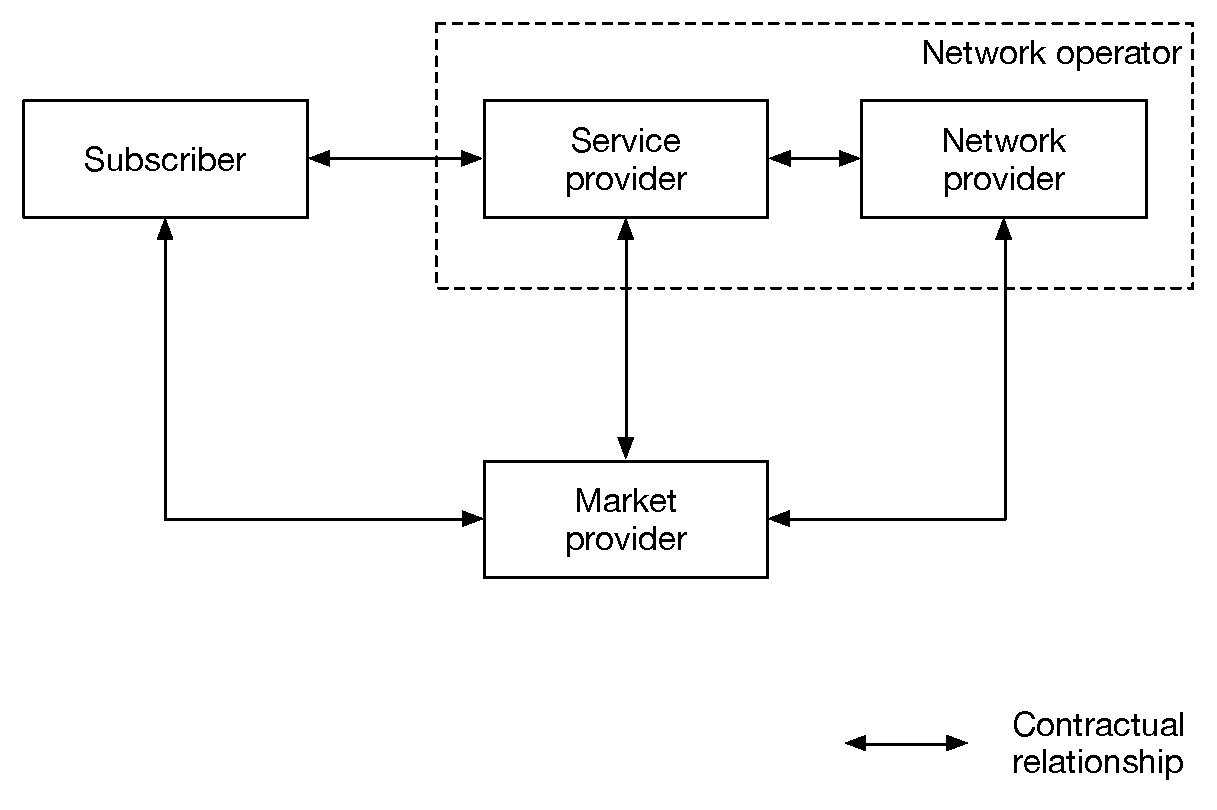
\includegraphics[width=4in]{DMP/Figures/dmp_model}
	\caption{The business model of Digital Marketplace (adapted from~\cite{DMIrvine02})}
	\label{fig:dmp_model_dmp}
	\vspace{10mm}
	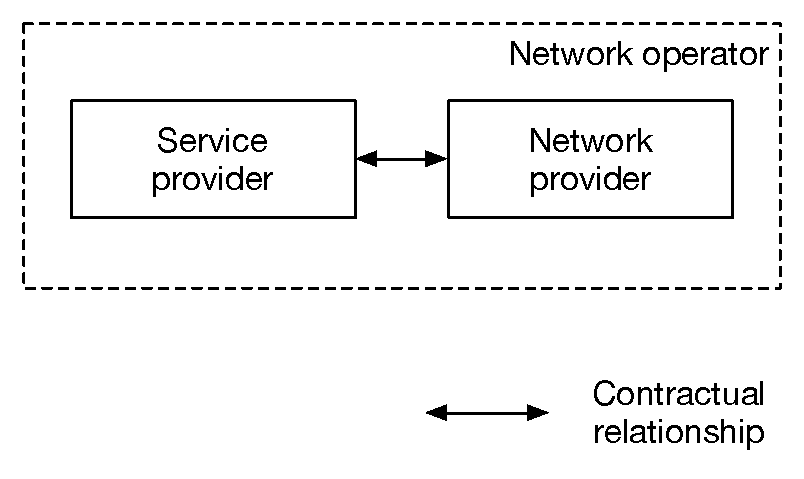
\includegraphics[width=5in]{DMP/Figures/no_decoupled}
	\caption{Decoupling of network operator into service and network providers (adapted from~\cite{DMIrvine02})}
	\label{fig:no_decoupled_dmp}
\end{figure}

It should be noted that the original specification of the DMP found for example in~\cite{DMLeBodic00,DMIrvine02,LeBodicThesis} differentiates between service and network providers. Thus, the network operator as an entity is decoupled into service and network providers as shown in Figure~\ref{fig:no_decoupled_dmp}. According to this model, the service provider is responsible for providing communications services to the end-user, while network provider facilitates (physical) network resources required to transport said services. A good example of a service provider is that of a mobile virtual network operator (MVNO). An MVNO, such as Giffgaff in the UK, provides services to the end-users, but does not necessarily own a physical network infrastructure; instead, they enter into a contract with an MNO, and use their network to transport users' services. In the UK, Giffgaff has such a contractual agreement with O2.

\annotate{C3.6}{While the original specification of the DMP advocates decoupling of service and network provision, the research reported in this thesis concentrates on the basic business model; i.e., service and network provision is handled by one entity, a network operator. The basic business model is seen as the most appropriate since any additional aspects of the decoupled case can later be incorporated into the mathematical model of the negotiation process developed in this thesis without affecting the results reported herein.} Nevertheless, all of the results presented in this thesis are applicable to the decoupled case. Indeed, it is a matter of replacing network operator with network provider; or replacing subscriber with service provider, and network operator with network provider. In the latter case, the negotiation process (or network selection mechanism which is described in Section~\ref{sec:network_selection_mechanism_dmp}) is between service and network providers. In this case, service provider acts as a buyer, while network providers are the sellers.

In this section, the principles of operation of the DMP were outlined. The next section provides a conceptual overview of the negotation process between the subscriber and the network operators. This process is termed \emph{network selection mechanism}, and is the means for the subscriber to select the network operator who reflects their service preferences best.
% section principles_of_operation_dmp (end)

\section{Network Selection Mechanism} % (fold)
\label{sec:network_selection_mechanism_dmp}
This section is organised as follows. Firstly, a high-level overview of auction theory is given, which is necessary to understand the fundamental assumptions governing the network selection mechanism in the DMP. Then, a conceptual overview of the network selection mechanism is provided.

\subsection{Primer in Auction Theory} % (fold)
\label{sub:primer_in_auction_theory_dmp}
As argued by many economists~\cite{Klemperer1999,Milgrom2004}, auction theory is one of the most prominent branches of economics. Examples of auctions being used in real life abounds: purchasing rare items of considerable value such as paintings, buying a house, or simply shopping on eBay. Another very good example of the popularity of auctions in real life is the well-known case of spectrum auctions which were used by both the US and the UK governments to sell the radio spectrum licenses to network operators. It is the purpose of this section to provide a high-level overview of the most important models and assumptions of auction theory.

\subsubsection{Common Auction Formats} % (fold)
\label{ssub:common_auction_formats_dmp}
\annotate{C3.10}{There are many different auction formats reported in the auction theory literature; however, four are particularly popular, and are explored in this section~\cite{Krishna10}.} Those are \emph{English} (also known as open ascending-price), \emph{Dutch} (also known as open descending-price), \emph{first-price sealed-bid}, and \emph{second-price sealed-bid} auctions.

\annotate{C3.10}{In an English auction, the person who conducts the sale, i.e., the auctioneer, calls out bids in an increasing fashion until there is only one interested bidder left~\cite{McAfee1987}.} For example, the sale of a painting (or other work of art) would traditionally be facilitated by the mechanism of an English auction. In such an auction, the auctioneer would set the base price for the object to be sold, $x$ say. Suppose further that some bidder A registered their interest (by raising their hand, or otherwise) in obtaining the object for the price of $x$. Then, bidder A would be proclaimed the highest bidder, and the auctioneer would call out another price, $y$, such that it is higher from the previous one, $x < y$ (hence, the alternative name of ascending-price auction). If other bidder, bidder B say, registered their interest in obtaining the object for the new price of $y$, then bidder B would become the highest bidder, and the auctioneer would further increase the price. And so on, until no further interest was observed. The object would then go to the current highest bidder.

\annotate{C3.10}{Similarly to an English auction, in a Dutch auction, the prices of the object for sale change in a sequential manner; however, in a Dutch auction, the price is decreasing~\cite{McAfee1987}.} The auction is conducted in the following way. The auctioneer starts at a price $x$, say. If no bidder registers interest within the given time limit set by the auctioneer, then the price is decreased to $y$, say, such that $y < x$. And so on, until a bidder registers interest. Then, the object is sold for that price to that bidder. It is worth noting that English and Dutch auctions are an example of open auctions since every bidder observes the bids of all the other bidders. This is in contrast to first-price and second-price sealed-bid auctions where bidders submit their bids simultaneously in sealed envelopes.

\annotate{C3.10}{In a first-price sealed-bid auction, the bidders submit their bids simultaneously in sealed envelopes to the auctioneer~\cite{McAfee1987}.} The bidder who submitted the highest bid, wins the auction and pays what they bid. Second-price sealed-bid auction is very similar to a first-price sealed-bid auction with this difference that the highest-bidding bidder wins the auction, but pays the amount equal to the second-highest bid. That is, suppose the highest and second-highest bids are denoted by $b_1$ and $b_2$ respectively such that $b_1 > b_2 > b_i$ for all $i$ such that $i > 2$. Then, in a first-price sealed-bid auction, bidder who submitted the highest bid $b_1$ wins and pays that amount. In a second-price sealed-bid auction, on the other hand, bidder who submitted the highest bid $b_1$ wins, but pays the amount equal to the second-highest bid $b_2$.
% subsection common_auction_formats_dmp (end)

\subsubsection{Bidder Valuations} % (fold)
\label{ssub:bidder_valuations_dmp}
The main reason for a seller of an object to use an auction mechanism is because they are uncertain how valuable the object is to the potential bidder. Otherwise, if the bidders' valuations were known, the seller would simply discriminate by offering the object to the bidder who is willing to pay the most~\cite{Krishna10}. This uncertainty in bidders' valuations is categorised into three distinct models: \emph{private values}, \emph{common values}, and \emph{interdependent values} model.

In private values model, each bidder knows the value of the object to himself at the time of bidding. Furthermore, each bidder can only make an intelligent guess about the valuations of other bidders. Finally, the knowledge of other bidders' valuations would not affect the bidder's own valuation for the object.

In common values models, the value of the object is the same for all bidders. It is, however, unknown to them at the time of bidding except for some estimates of the true value.

The interdependent values model generalises the common values model in the sense that the value of the object is not necessarily the same for all bidders. The bidders, however, still possess only estimates of the true value of the object at the time of bidding. Furthermore, in interdependent values model, the information available to other bidders, i.e., their estimates of the value, may influence the value of the remaining bidders if known to them.

To put the models in context, a scenario where a painting is sold at an auction and the bidders do not intend to resell the object in the resale market, that is, they assign values to a painting only on the basis of how much utility they would derive from possessing it, can accurately be approximated by private values model. Common values and interdependent values model, on the other hand, is a good approximation to an auction where land with an unknown amount of oil is being sold; bidders may possess different estimates of the amount of oil, but the final value depends directly on the future sales of the extracted oil.
% subsection bidder_valuations_dmp (end)

\subsubsection{Standard versus Procurement Auctions} % (fold)
\label{ssub:standard_versus_procurement_auctions_dmp}
So far, only the assumptions and models of auction theory where a number of bidders is contesting for the right to buy an object were discussed. However, auctions can also be used to sell goods. In other words, in such a scenario, the auctioneer is trying to purchase an item for the lowest price from a set of sellers/bidders. This type of auctions is referred to as \emph{procurement auctions}.

It is important to realise that, from a game-theoretical perspective, procurement auctions are equivalent to standard auctions in the same setting~\cite{Krishna10}. Therefore, the abundance of results on standard auctions applies to procurement auctions with only certain small, conceptual differences; for example, standard auctions consider the maximum bid, while procurement auctions the minimum bid. This fact is exploited in this thesis, and proofs of the results not already covered in the literature on auctions in general are provided. This is since if the result is proved in one case (be it either for standard or procurement auctions), it can immediately be adapted to the other case.

To provide an example, consider a procurement first-price sealed-bid auction. First-price auction is discussed since, as evident in the subsequent section, the network selection mechanism in the DMP is based on a procurement first-price sealed-bid auction. Similarly to the standard auction, the bidders (sellers of a good) submit their bids (prices) simultaneously in sealed envelopes to the auctioneer (buyer). Suppose the lowest and second-lowest bids are denoted by $b_1$ and $b_2$ respectively such that $b_1 < b_2 < b_i$ for all $i$ such that $i > 2$. Then, the bidder who submitted the lowest bid $b_1$ wins the auction, and sells the good to the auctioneer for the price equivalent to their bid, i.e., $b_1$.
% subsection standard_versus_procurement_auctions_dmp (end)
% subsection primer_in_auction_theory_dmp (end)

\subsection{Conceptual Overview} % (fold)
\label{sub:conceptual_overview_dmp}
The process of negotiation (or the network selection mechanism) in the DMP is based on a procurement first-price sealed-bid auction. Unlike in a procurement first-price sealed-bid auction, however, the winning bid is a weighted (convex) combination of both the network operator's monetary bid and their reputation rating; henceforth referred to as the \emph{compound bid}. The network operator is elected as the winner of the auction if their compound bid is the lowest in value, and accrues their monetary bid minus the cost of supporting the service. The monetary bid is equivalent to the price of supporting the service by the network operator. The precise definition of the price is left open-ended; one possibility, for example, would be to charge the buyer per unit of bandwidth. The weights in the compound bid are set by the subscriber before each auction, and are announced to the network operators. This effectively gives the subscriber the freedom to choose any combination ranging from: a low price for the service but also poor quality; to a high quality but for a high price \cite{DMLeBodic00}.

It is important to note that, out of sequential-bid and sealed-bid auctions, a procurement first-price sealed-bid auction was chosen due to the following reasons. Firstly, given the timing constraints in the DMP (e.g., the waiting time of the subscriber for the service to be admitted), and the difficulty in predicting the number of bids placed until the winner is selected in a sequential-bid auction, sealed-bid auctions were deemed as the most appropriate~\cite{DMLeBodic00}. Secondly, the rules governing a second-price sealed-bid auction may appear as counter-intuitive to the subscriber; that is, as mentioned in the previous section, the lowest bid secures the auction but the price paid equals the second-lowest bid. Lastly, since the subscribers not only base their network selection strategy on the offered price, but also on reputation, a first-price sealed-bid auction is the best fit to such a requirement.

Furthermore, since the communications services are traded on an individual service level, it might be difficult for the subscriber to judge the overall quality of the services supplied by a particular network operator \cite{DMIrvine02}. Therefore, one of the fundamental assumptions governing the operation of the DMP is that, by registering in the DMP, network operators agree to report on their contract fulfillments to the market provider; that is, they agree to report a binary value denoting the success in delivering the service to the subscriber within the agreed QoS bounds \cite{DMLeBodic00}. The value of $0$ denotes a failure, while the value of $1$ a success. The latest $d$ ($d>1$) reports are then used to compute the reputation rating of the network operator which will be used when a new service request arrives in the marketplace. Hence, assuming network operator $i$ admitted $t$ service requests, the formula for computing a reputation rating update is as follows (cf.~Section~3.2 in~\cite{DMLeBodic00})\annotate{C3.1}{
\begin{equation}
    \label{eq:reputation_rating_update_dmp}
    r_i^{t+1} = \sum_{k = t-d}^d \frac{1 - \rho_i^k}{d},
\end{equation}
where $\rho_i^k$ denotes the $k^{\text{th}}$ binary report of the network operator $i$.} \annotate{C3.4}{It is important to notice that the reputation rating relates to the network operator rather than to the type of service offered by the network operator, such as phone call, email or web browsing requests~\cite{LeBodicThesis}.} Note further that Equation~\eqref{eq:reputation_rating_update_dmp} implies $r_i^{t+1} = 0$ if the network operator $i$ has successfully delivered $d$ services to the subscriber, while $r_i^{t+1} = 1$ if has failed in all $d$ attempts. Furthermore, Equation~\eqref{eq:reputation_rating_update_dmp} implies that if the operator is consistently unreliable, their performance is reflected accordingly by their reputation rating history. Whilst, similarly, one failure in delivering the service does not immediately render a network operator unreliable; rather, it marginally affects their updated reputation rating. At the same time, at the end of each contract, the subscriber may report on their satisfaction (or Quality of Experience, QoE) with the service, for example, by submitting a mean opinion score in case of real-time services, and achieved throughput for non-real-time ones. The reputation rating update formula in Equation~\eqref{eq:reputation_rating_update_dmp} could then be modified to incorporate QoE, for instance, by taking an appriopriately weighted composition of both network operator's and subscriber's reports. Since this section just barely scratches the surface of the reputation rating system maintained by the DMP, and the concept of QoE, the readers are referred to \cite{DMLeBodic00,DMIrvine01,DMIrvine02,LeBodicThesis,DMMathur02,DMMcDiarmid06} for a more in-depth treatment of the former and to~\cite{Kilkki2008, BrooksHestnes2010, Fiedler2010, Shaikh2010} of the latter.

In this section, a conceptual overview of the network selection mechanism was provided. The next section outlines the contributions of the research reported in this thesis to the DMP.
% subsection conceptual_overview_dmp (end)
% section network_selection_mechanism_dmp (end)

\section{Previous Research on the Digital Marketplace} % (fold)
\label{sec:previous_research_on_the_digital_marketplace_dmp}
In this section, previous research on the DMP is summarised.

Over the last two decades, several papers have explored both the economic and technical challenges of the DMP. In their seminal paper, Le Bodic \emph{et al.}~\cite{DMLeBodic00} discuss how the DMP can be used in a 3G environment to increase the competition between network operators by using a marketplace approach. Furthermore, they describe the business and technical underpinnings of the DMP. Finally, the operation and the fundamental assumptions of the network selection mechanism are outlined, and a bidding strategy based on a tatonnement process is proposed. The tatonnement process is based on the principle that each network operator analyses past auctions in order to determine the market price they have to offer to remain competitive. The DMP is then simulated with the proposed bidding strategy as the equilibrium bidding strategy, and the evolution of the market equilibrium is analysed under different simulated scenarios. \annotate{C3.2}{It is worth noting that the ideas presented in Le Bodic's paper~\cite{DMLeBodic00} are substantially extended and elaborated upon in Le Bodic's PhD dissertation~\cite{LeBodicThesis}.}

Irvine \emph{et al.}~\cite{DMIrvine01} explore the problem of interconnection between DMPs. More specifically, they examine how, in a hybrid environment featuring a variety of wireless access technologies, service requests are handled between multiple DMPs, e.g., call interconnections. Simulation results for four interconnected DMPs are presented, and the bidding mechanism proposed in~\cite{DMLeBodic00} is simulated. It is concluded that with that bidding strategy in force, network operator should accept as many calls as possible, and let the quality of the service degrade. The paper then concludes with the statement that since the DMP is a complex system, many different bidding strategies may be used, but complex bidding strategies are not necessarily beneficial.

In~\cite{DMIrvine02}, Irvine describes in detail the business model for the DMP, and presents the fundamental requirements for a market to operate freely. He then highlights how the DMP fulfils all the requirements thus establishing DMP a free market. Finally, he summarise the operation of the DMP, discusses how DMP can be used as a management platform for services beyond 3G, and draws a comparison between DMP and other similar solutions.

Mathur \emph{et al.}~\cite{DMMathur02} propose a method for accurate estimation of reputation ratings. They derive a 3D surface graph which allows the network operators to deduce how many users they can accomodate in the network before they reach limits in capacity, and as a result, risk degrading their reputation. The 3D surface is derived through the means of simulation modelling, and encapsulates three categories of users: voice heavy users, data (mainly web browsing) heavy users, and video heavy users.

In~\cite{DMMcDiarmid06}, McDiarmid \emph{et al.}~extend the reputation system of the DMP by introducing a new parameter called commitment level as a means of securing the DMP. This parameter is meant to encapsulate the commitment of the network operators to successfully providing the required QoS levels of a service as requested by the subscriber. That is, if a network operator sets their commitment level at 90\%, then they declare that they will strive to fulfil at least 90\% of all the contracts (within a time window) to their required QoS levels. The authors simulate their proposed reputation system, and conclude that it is fair towards network operators; that is, it rewards providers who exceed their commitment level, and punishes those who fail.

Finally, in~\cite{DMBushTussle09}, Bush \emph{et al.}~extend the ideas presented in~\cite{DMIrvine02} to next generation wireless networks; that is, a wireless environment featuring a plethora of wireless access technologies, such as 3G, 4G and beyond. The authors argue that the DMP can be used to manage the effect of a `tussle' in the next generation wireless networks. They predict the tussle between different economic agents involved, and especially between the end-users of wireless service, service and network providers.

In this section, previous research on the DMP was summarised. The next section outlines the contributions of this research to the DMP.
% section previous_research_on_the_digital_marketplace (end)

\section{Contributions of this Research to Digital Marketplace} % (fold)
\label{sec:contributions_of_this_research_to_digital_marketplace_dmp}
Out of six papers presented in the previous section, only two papers~\cite{DMLeBodic00,DMIrvine01} touch upon the issue of the best bidding strategy for the network operators. In both cases, the bidding strategies are given as is rather than being a result of an in-depth economic/game-theoretical analysis. The work reported in this thesis addresses this issue by providing a comprehensive analysis of the network selection mechanism from the economic viewpoint. As such, bidding strategies that constitute an equilibrium of the auction upon which the network selection mechanism is based are characterised. In this context, the equilibrium bidding strategies are equivalent to the best bidding strategies network operators can undertake. Furthermore, it is shown that the equilibrium exists and it is unique, and can be approximated numerically.
% section contributions_of_this_research_to_digital_marketplace_dmp (end)

\section{Summary} % (fold)
\label{sec:summary_dmp}
In this chapter, the concept of the DMP was introduced, and an outline of the fundamental assumptions and operation of the network selection mechanism employed by the DMP was provided. The chapter then concluded with a summary of previous research on DMP, and an explanation of how the research work reported in this thesis contributes to the DMP framework.
% section summary_dmp (end)
% chapter digital_marketplace_dmp (end)